\documentclass[a4paper,12pt]{report}
\usepackage[utf8]{inputenc}
\usepackage[italian]{babel}
\usepackage[italian]{cleveref}
\usepackage{anyfontsize}
\usepackage{fancyhdr}
\usepackage{changepage}
\usepackage{geometry}

\usepackage{booktabs} % For prettier tables
\usepackage{graphicx}
\usepackage{array}
\usepackage[table]{xcolor}
\usepackage[section]{placeins}
\usepackage{float}
\usepackage{tabto}
\usepackage{comment}
\usepackage{listings}
\usepackage{color}

\definecolor{Rosso}{gray}{0.9}

\pagestyle{fancy}
\fancyhf{}
\rhead{Overleaf}
\lhead{Guides and tutorials}
\rfoot{Page \thepage}
\usepackage{fancyhdr}
\usepackage{lipsum} % only for showing some sample text
\fancyhf{} % clear all header and footers
\renewcommand{\headrulewidth}{0pt} % remove the header rule
\rfoot{\thepage}


\title{Relazione\break``progetto FormulaDB''}
\author{Migliarini Gianluca - Montali Giacomo}
\date{Giugno 2021}

\begin{document}	
	\maketitle
	%Chapter Analisi ---> controllo analisi
	%Chapter logica  ---> elenchi puntati
	\chapter{Analisi dei requisiti}
		\section{intervista}
		{\fontsize{12.5}{20}\selectfont
		Si vuole tenere traccia dei campionati del mondo Formula, memorizzando per ciascuno l'anno del campionato e la categoria di auto che corre al suo interno.
		In ogni campionato gareggiano circa 20 piloti, dei quali vengono salvate informazioni come il nome ed il cognome del concorrente,
		la nazionalità, la data di nascita ed il numero con il quale corre.
		Per poter gareggiare, ogni pilota stipula un contratto con una scuderia, la quale gli offre un veicolo, con il quale
		prendere parte alle competizioni. Il contratto ha solitamente durata di qualche anno, tuttavia, in rare occasioni,
		la scuderia permette al pilota di gareggiare per un team diverso.
		Per ogni scuderia si tiene traccia del suo nome e la nazione di provenienza.
		I test effettuati durante il periodo di pausa tra le varie competizioni, eseguiti da ingegneri specializzati appartenenti al team,
		permettono alla scuderia di migliorare la propria autovettura, offrendo così la possibilità di gareggiare
		con un nuovo modello per il campionato che verrà. In particolare, le migliorie apportate interessano il peso e le dimensioni dell'auto.
		Inoltre, le scuderie, in caso di budget ridotto, possono eventualmente acquistare il motore da team avversari.
		Per ogni scuderia è necessario tenere traccia degli ingegneri che ci lavorano e della loro specializzazione.
		Di ogni Gran Premio viene memorizzato, oltre alla data, il numero di giri ed il meteo;
		la posizione ed il nome del circuito dove viene disputato.
		Per quanto riguarda i circuiti, è necessario permetterne la localizzazione salvando il nome, la nazione e la città in cui sono situati.
		Inoltre, per una memorizzazione migliore di ogni gara, viene memorizzato ogni giro di ogni pilota effettuato in gara con il rispettivo tempo,
		i pit-stop effettuati con il tempo impiegato in essi, l'ordine di partenza (dato dalle qualifiche) e l'ordine di arrivo.}
	\newpage
	\chapter{Progettazione concettuale}
		\section{Scuderia e veicoli}
	{\fontsize{12.5}{20}\selectfont
	Per ogni campionato, le scuderie schierano il veicolo derivato dalle migliorie ingegneristiche apportate al modello
	precedente. Per regolamento una scuderia può offrire ai suoi piloti solamente un modello di veicolo per campionato.
	L'unica parte dell'automobile che in molti casi non è progettata dalla scuderia è il motore, il quale può essere
	acquistato da un team avversario, e, a differenza delle altre componenti, non può essere modificato ad ogni campionato.
	Un campionato si svolge in più gare, ognuna delle quali prende parte in un circuito ad una certa ora e con un numero
	di giri variabile, deciso dagli organizzatori in base a diversi fattori, quali l'orario e le condizioni meteorologiche; ragione per la quale, ogni Gran Premio viene identificato dal nome del circuito e dalla data e ora del suo svolgimento, in quanto nella stessa giornata possono avvenire più gare sulla stessa pista.}
	\pagebreak
	\begin{center}
		\hspace*{-2cm}%
		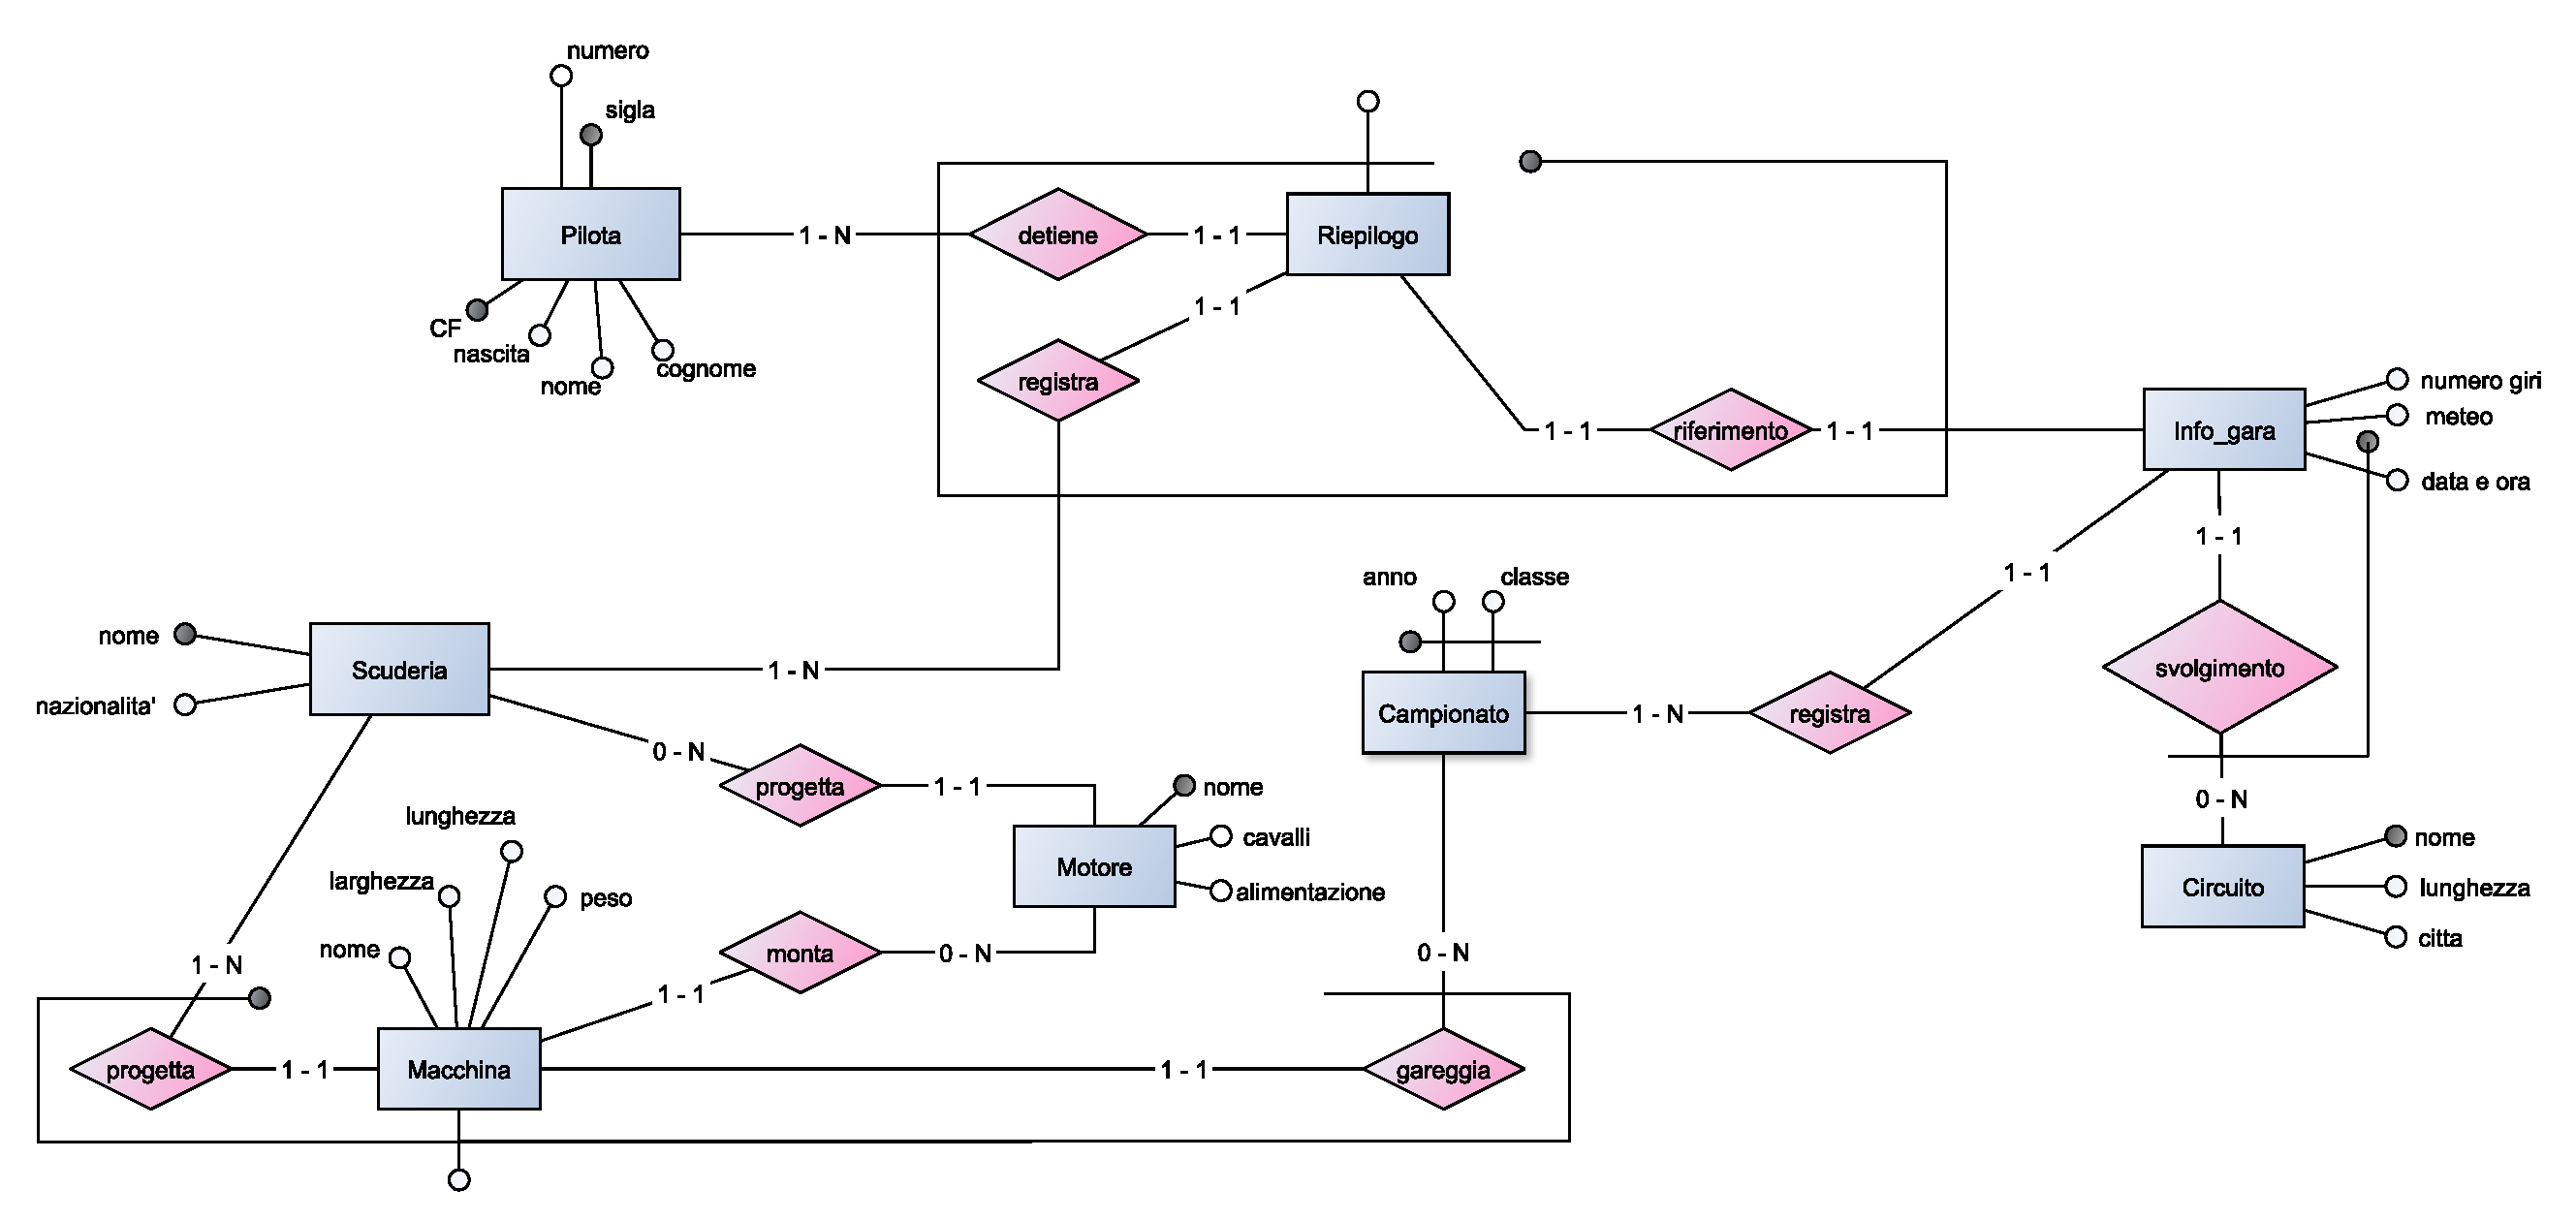
\includegraphics[width=\dimexpr\textwidth+10cm\relax, height=15cm, angle=90]{copies/scheletro2.pdf}%
		\hspace*{-4cm}%
	\end{center}
	\pagebreak
		\section{Piloti, ingegneri e contratti}
			{\fontsize{12.5}{20}\selectfont
			Le entità Pilota e Ingegnere ereditano gli attributi dal padre 'Persona', il quale tiene traccia dei
			dati anagrafici e viene identificato tramite il Codice Fiscale.\\
			Dell'entità ingegnere inoltre teniamo traccia della specializzazione.\\
			Per una migliore rappresentazione dei dati e per evitare casi di omocodia, il pilota viene identificato
			da una sigla, formata dalle prime tre lettere del cognome. In caso di sigle identiche, è compito della
			Federazione Internazionale dell'Automobilismo di scegliere un'abbreviazione adeguata al concorrente
			per evitare duplicati.\\
			Mentre un ingegnere stipula un contratto con una scuderia per tutta la durata della sua carriera,
			solitamente i contratti con i piloti sono di durata determinata.}
			\begin{center}
			\hspace*{-2cm}%
			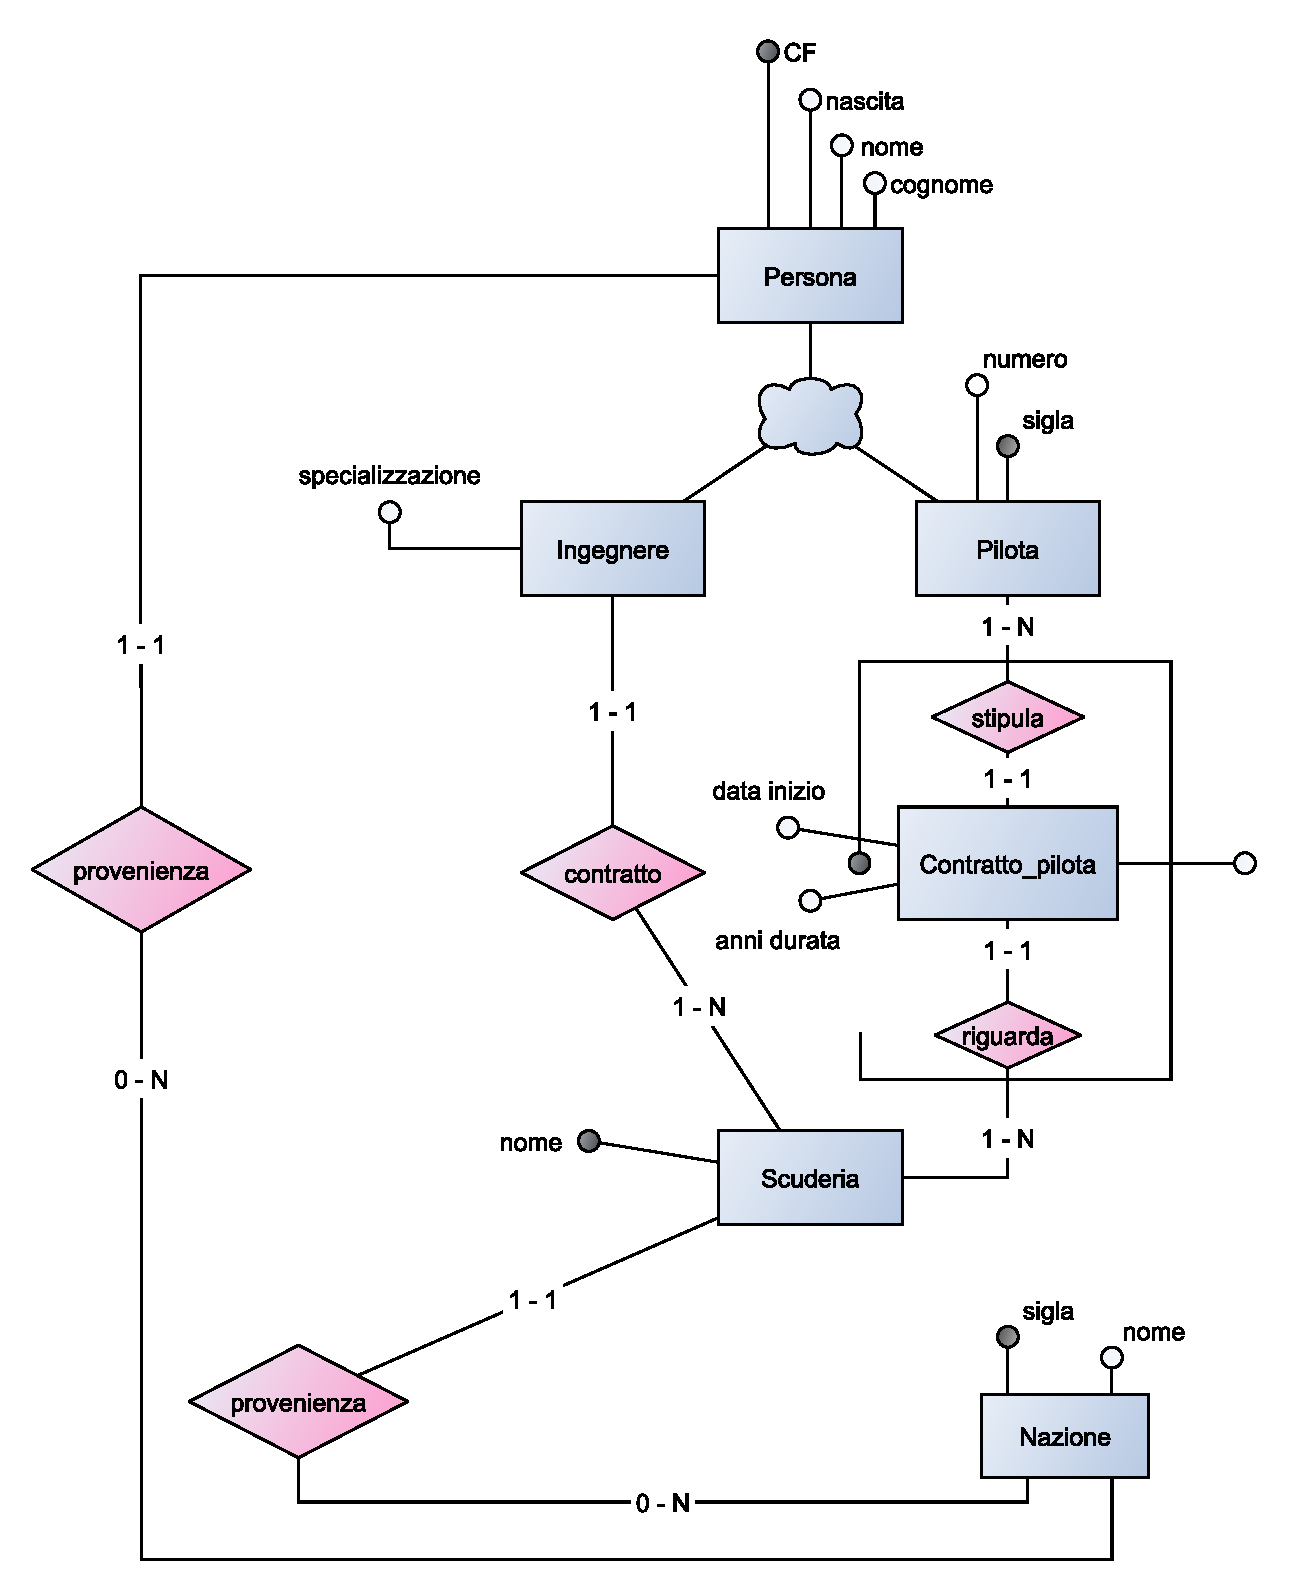
\includegraphics[width=\dimexpr\textwidth+4cm\relax]{copies/scheletro1.pdf}%
			\hspace*{-2cm}%
			\end{center}
		\pagebreak
		\section{Risultati}
	{\fontsize{12.5}{20}\selectfont
	Il risultato di un pilota in una gara viene memorizzato tramite l'entità Riepilogo.
	I giri, i pit-stop ed i risultati delle gare e delle qualifiche si collegano a Riepilogo tramite chiavi esterne.
	Ogni pilota può avere solamente un Riepilogo relativo ad una gara.
	Nonostante i vincoli derivanti dal contratto tra pilota e team, in casi rari, ai driver viene data la possibilità
	di partecipare ad una gara con una scuderia diversa da quella con la quale ha stipulato il contratto.}
	\newline
	\begin{center}
		\hspace*{-3cm}%
		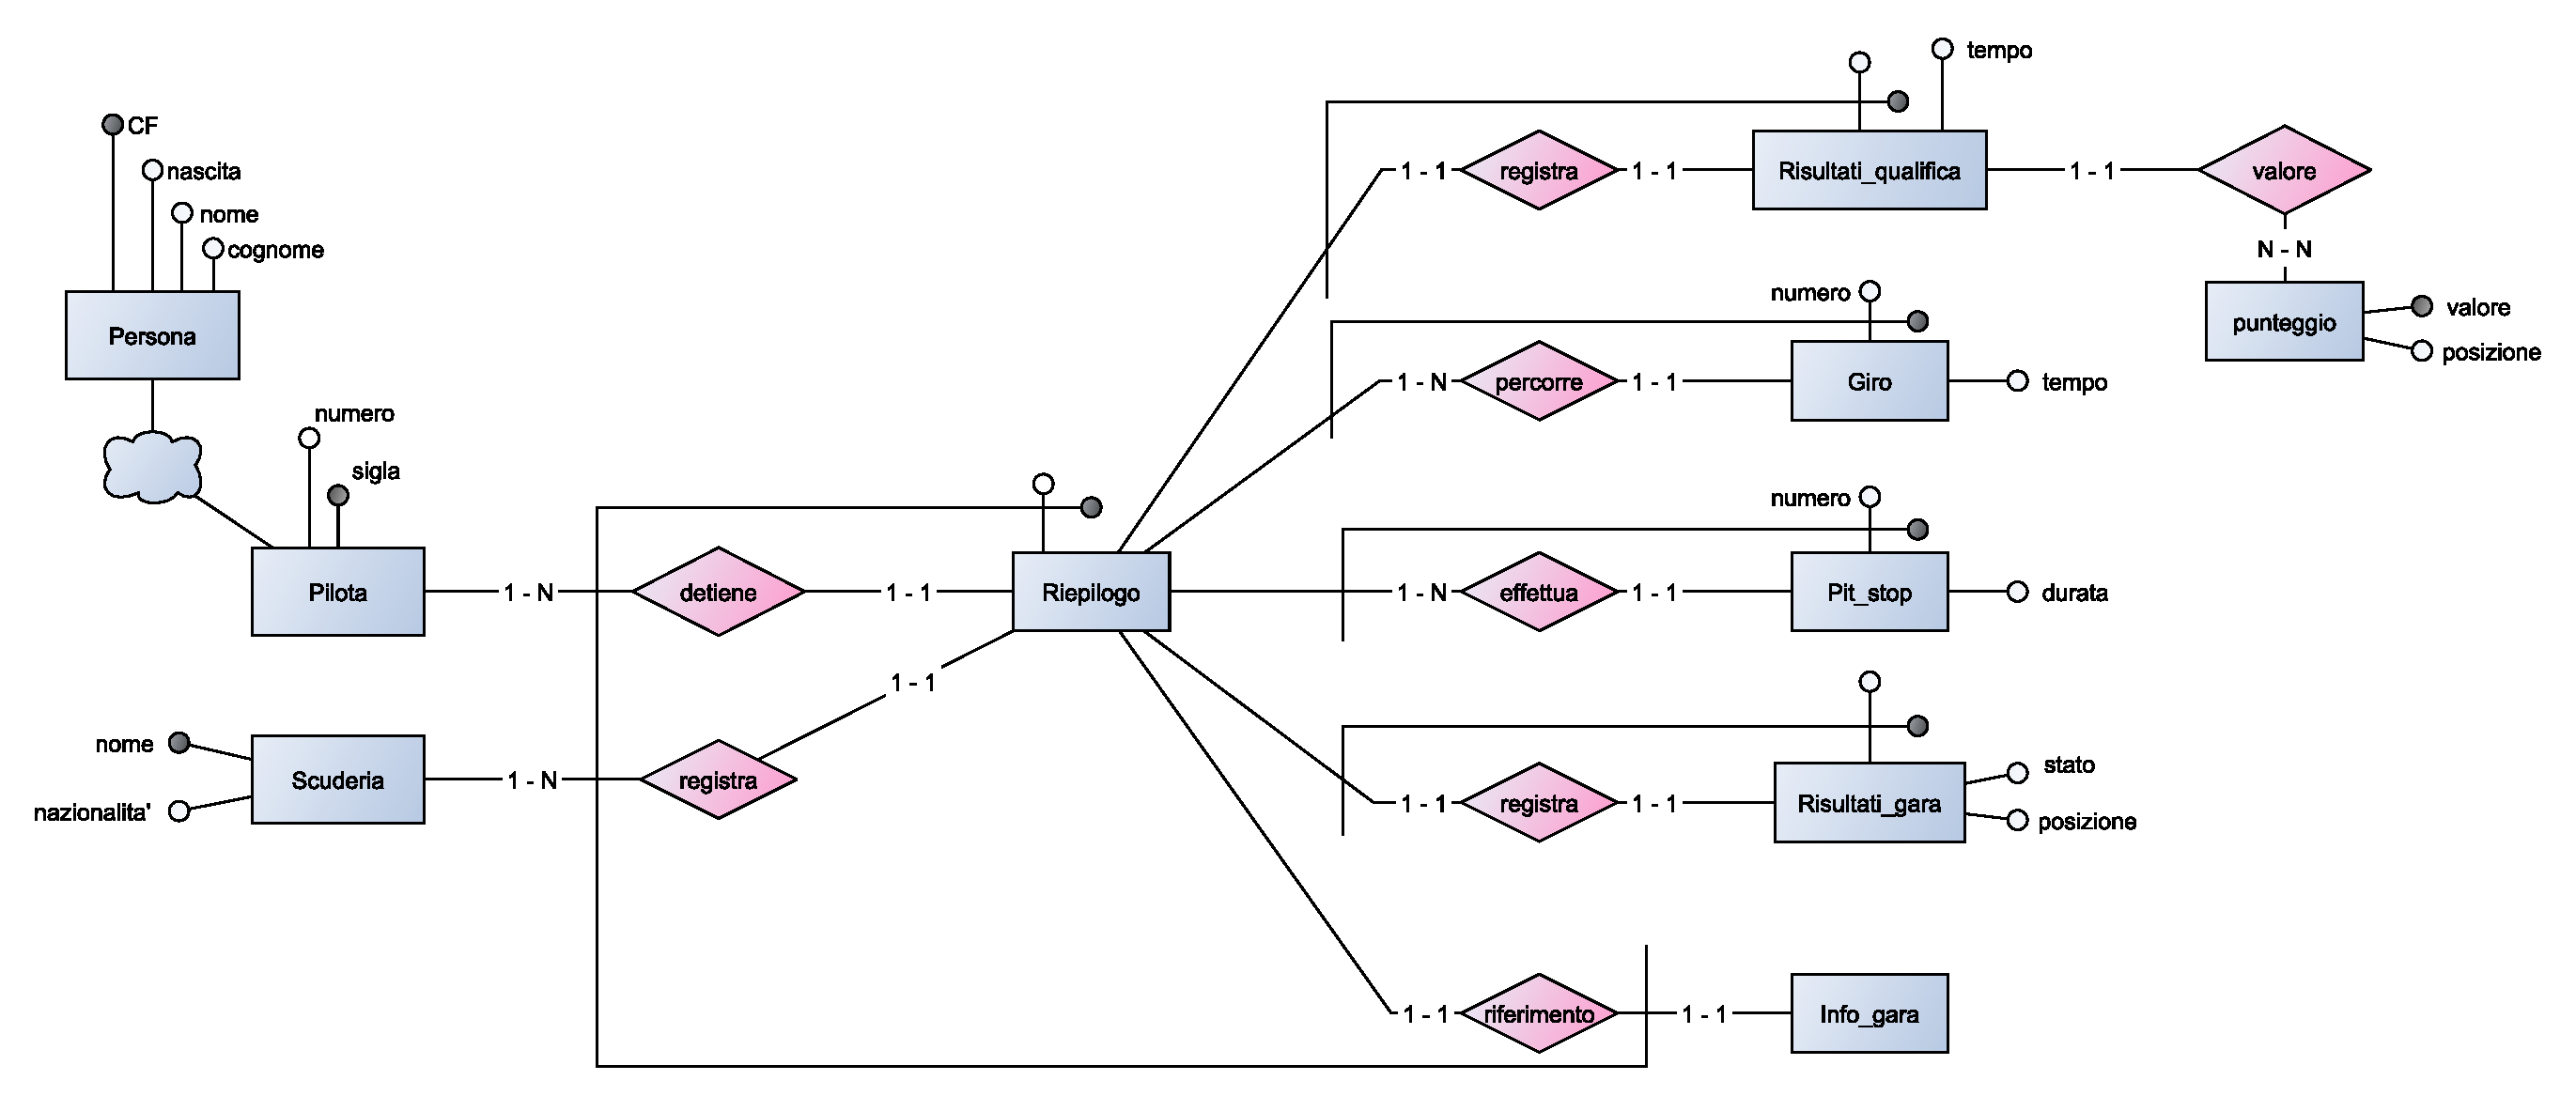
\includegraphics[width=\dimexpr\textwidth+6cm\relax, height=10cm]{copies/scheletro3.pdf}%
		\hspace*{-3cm}%
	\end{center}
	\pagebreak
		\section{Schema concettuale finale}
		\bigskip\bigskip\bigskip 
		\begin{center}
				\hspace*{-3cm}%
				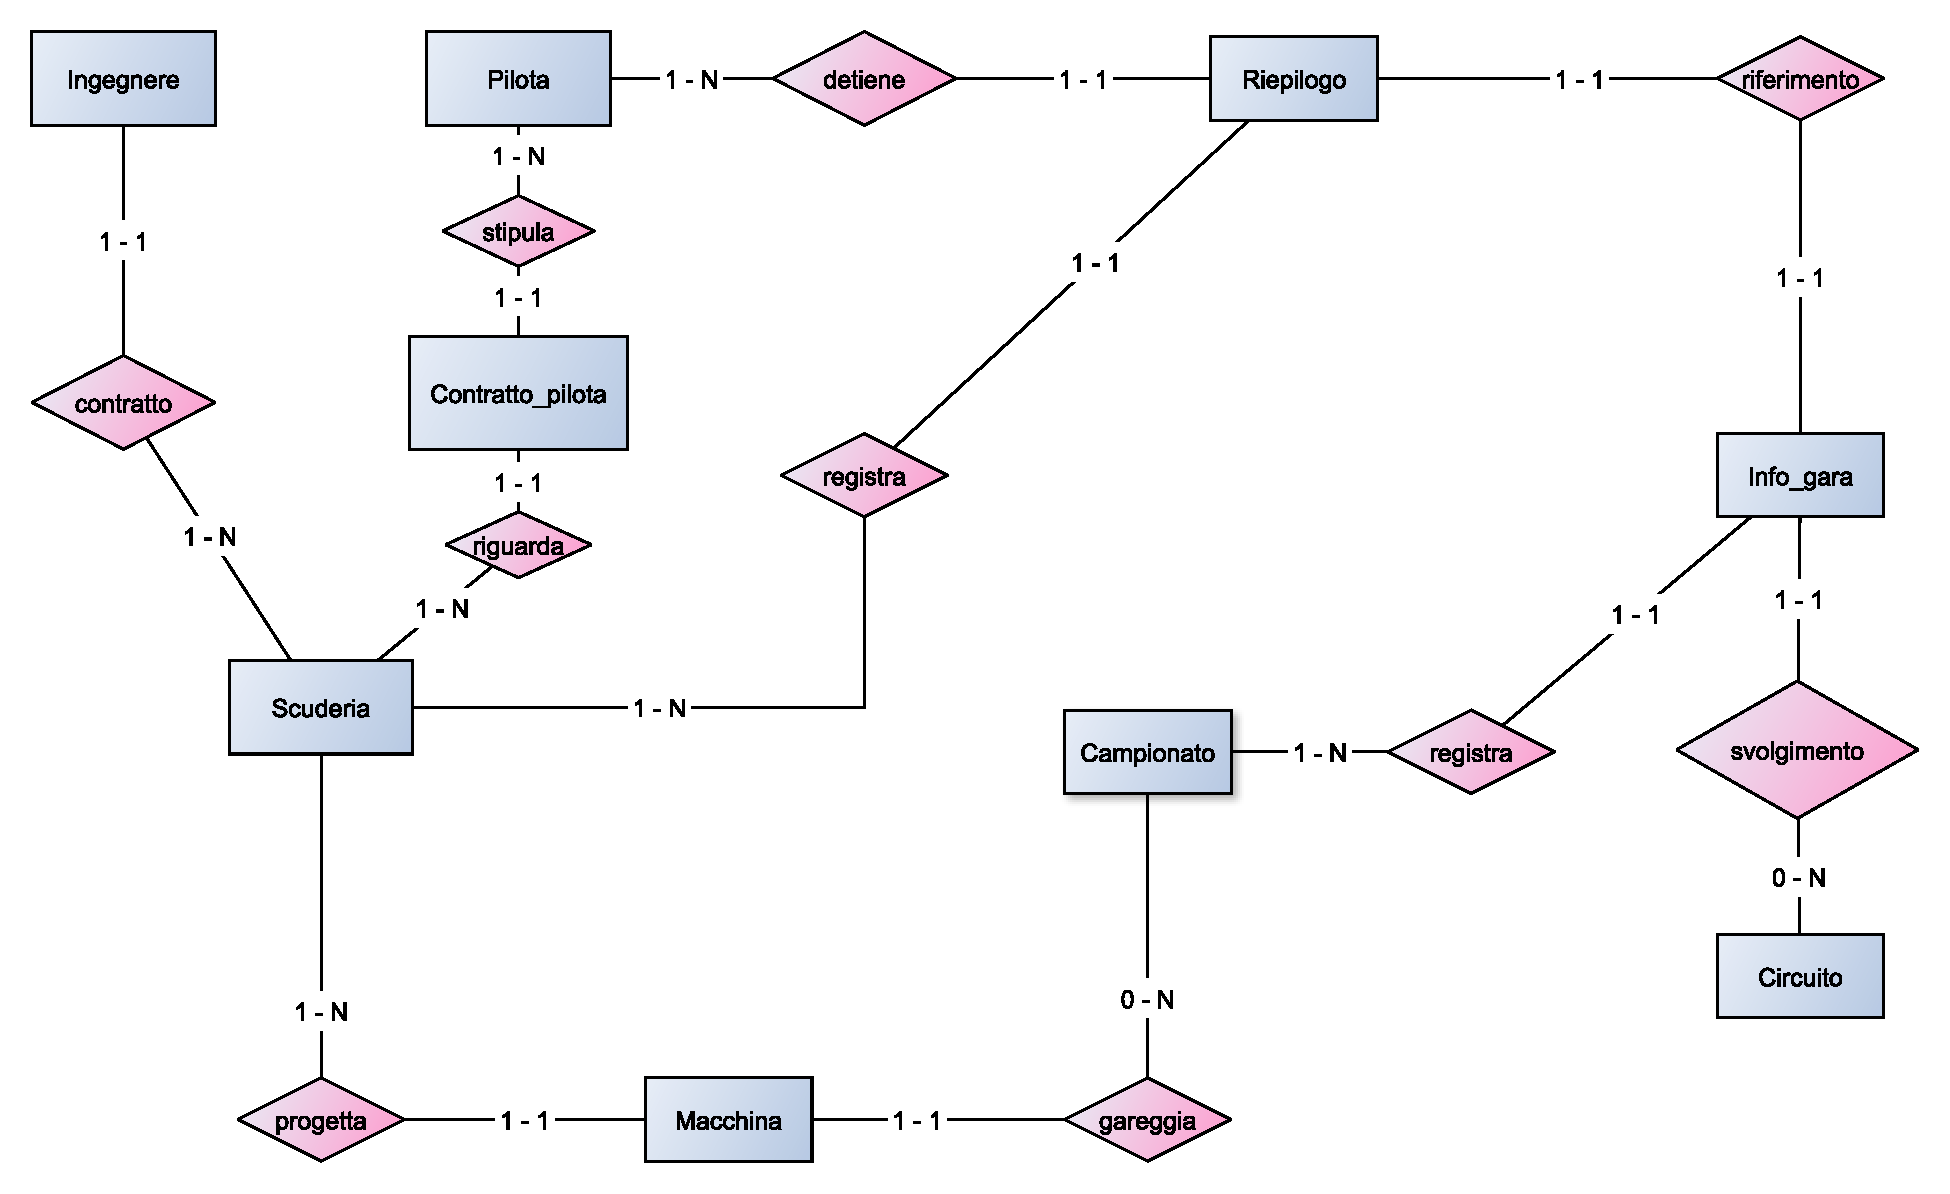
\includegraphics[width=\dimexpr\textwidth+6cm\relax, height=10cm]{copies/scheletrone.pdf}%
				\hspace*{-3cm}%
			\end{center}
		\pagebreak
		\section{Schema E-R finale}
		\begin{center}
				\hspace*{-2cm}%
				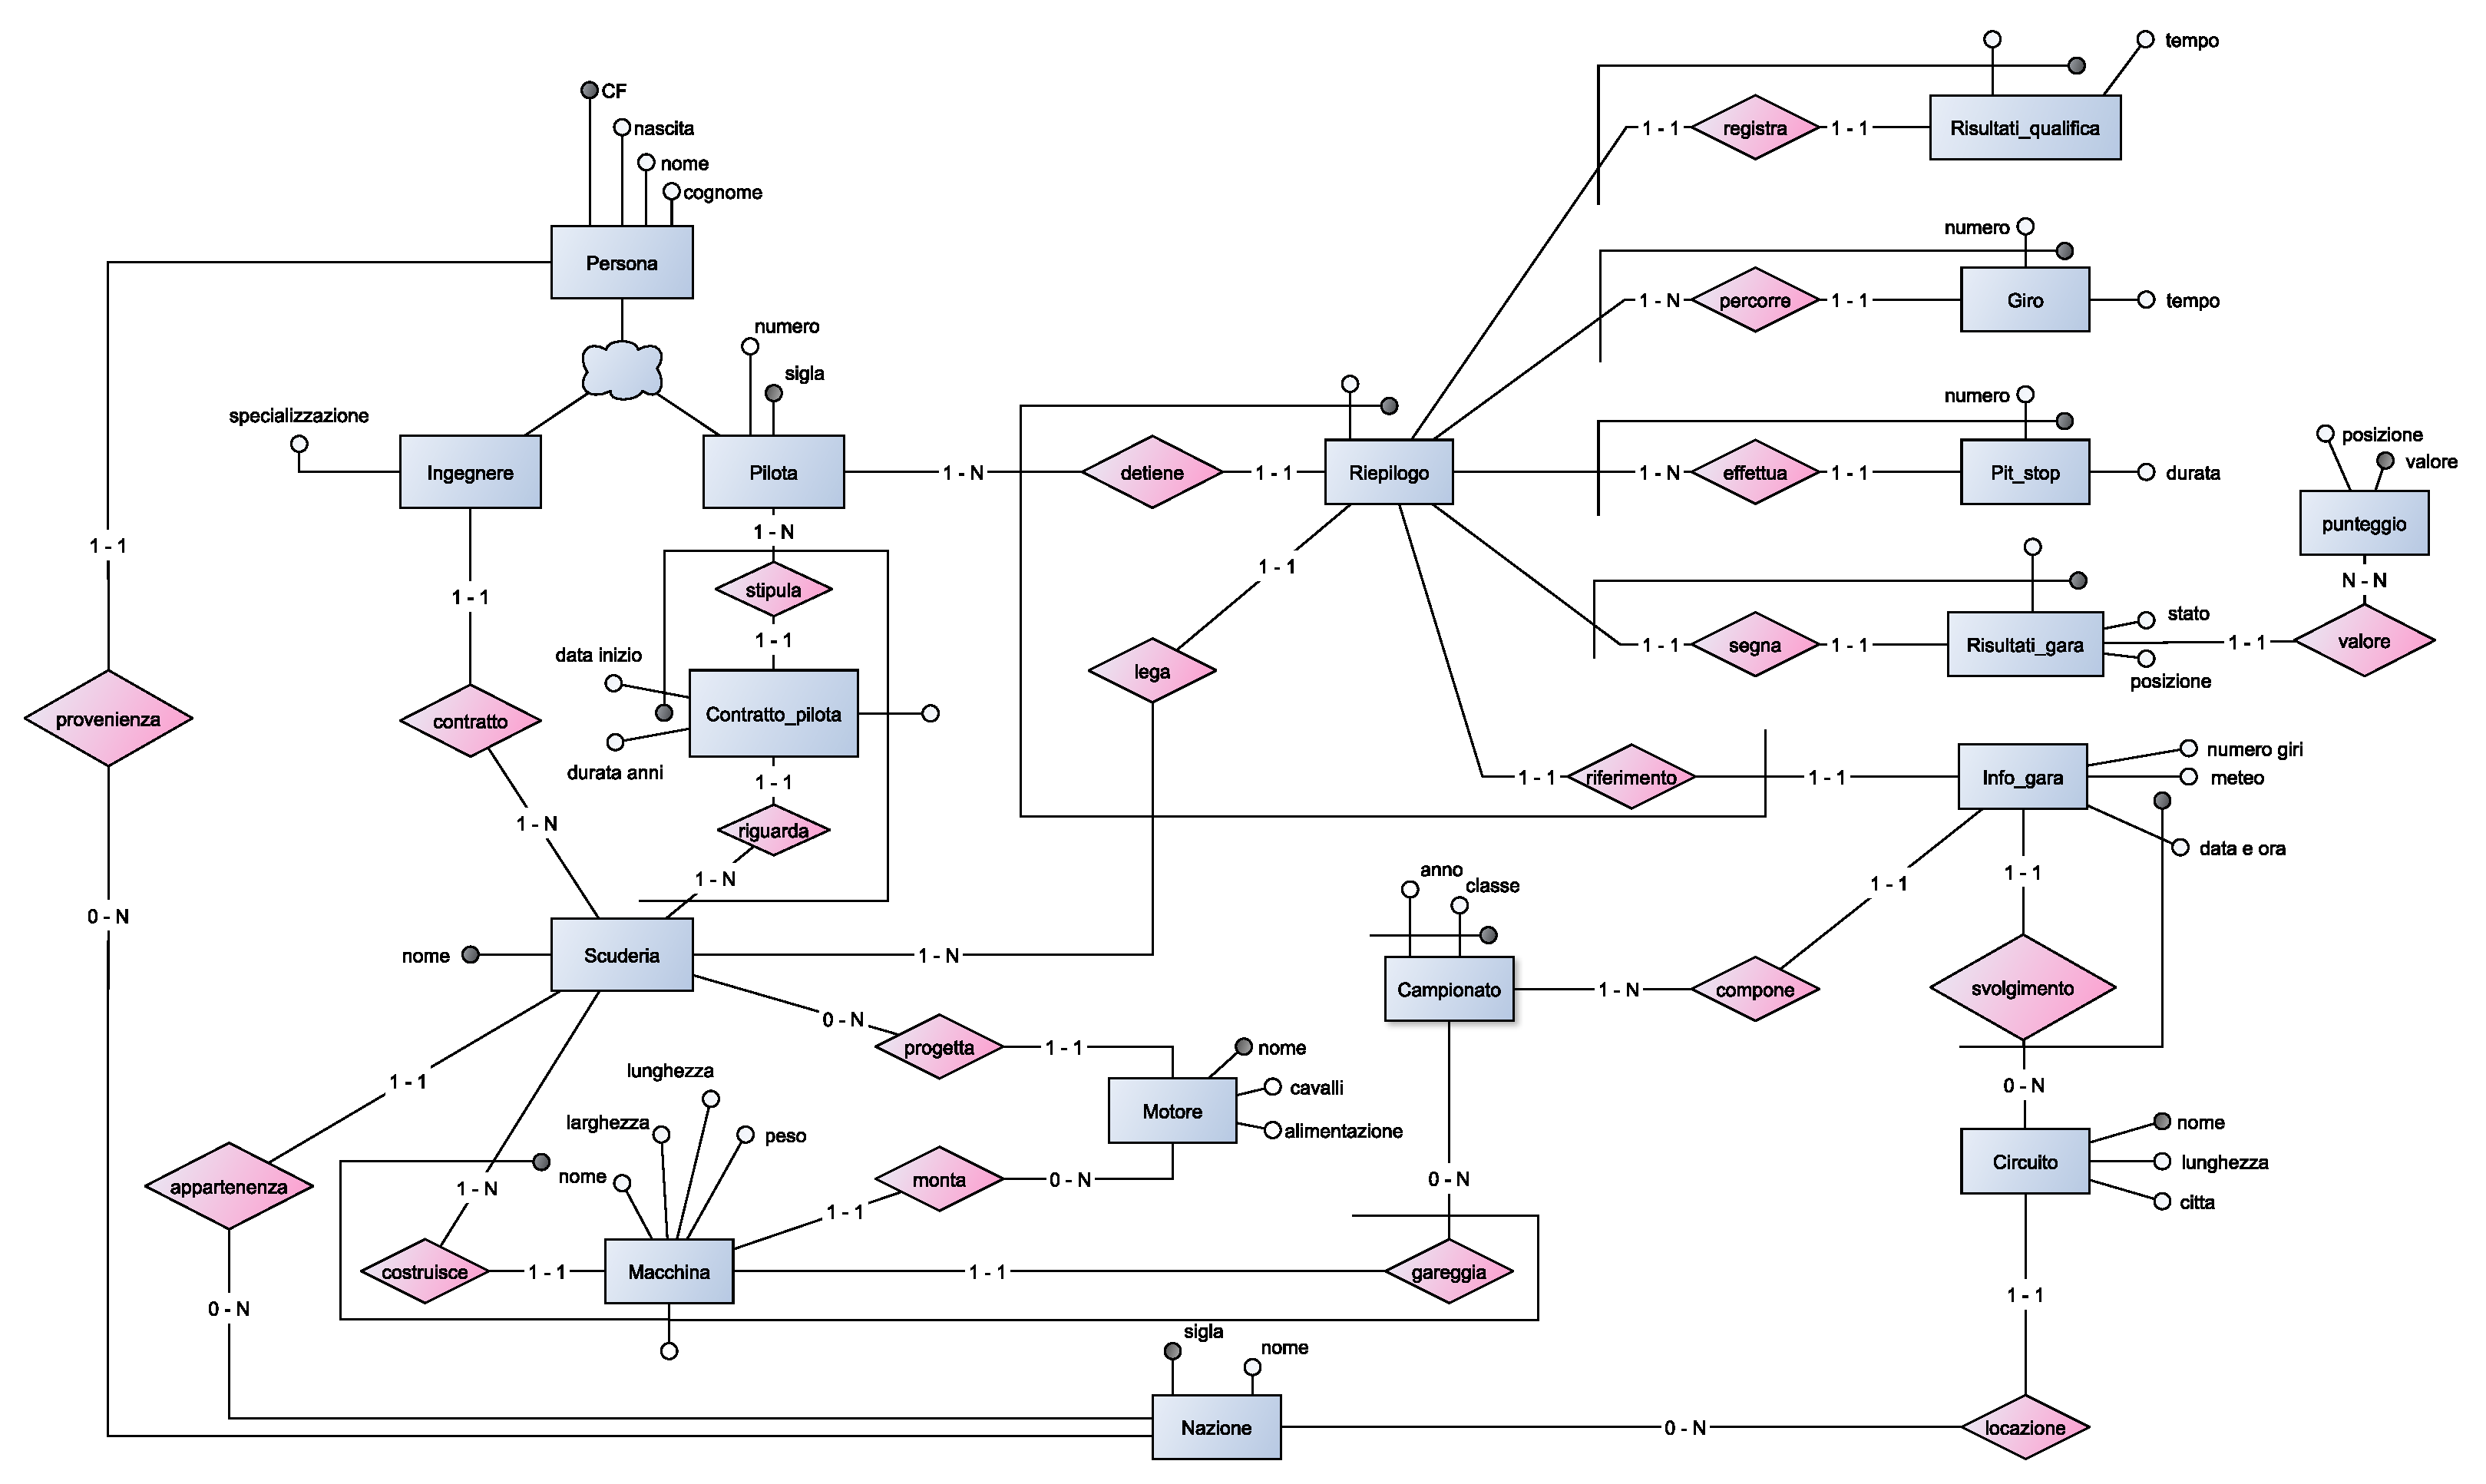
\includegraphics[width=\dimexpr\textwidth+6cm\relax, height=17cm, angle=90]{copies/ERfinale.pdf}%
				\hspace*{-8cm}%
			\end{center}
		\pagebreak

	\chapter{Progettazione logica}
		\section{Stima volume dati}
			\small\addtolength{\tabcolsep}{+10pt}
			\begin{table}[h!]
				\centering
				\begin{center}
					\label{tab:table1}
					
					\scalebox{1.3}{
					\begin{tabular}{|c|c|c|} % <-- Alignments: 1st column left, 2nd middle and 3rd right, with vertical lines in between
						%\toprule
						\hline\rowcolor{Rosso}
						\textbf{Dato} & \textbf{Tipo} & \textbf{Quantità}\\
						\hline\hline
						%\midrule		
						Nazione				&	E	&	210\\     
						Circuito			&	E 	&	100\\
						scuderia			&	E	&	40\\
						Pilota				&	E	&	110\\
						contratto\_pilota	&   R 	&	365\\
						Ingegnere			&	E 	&	2200\\
						Contratto			&	R 	&	2200\\
						Campionato			&	E	&	15\\	     
						Giro 				&	E 	&	360000\\
						info\_gara			&	E   &	300\\ 
						riepilogo			&	R	&	6000\\
						risultati\_gara		&	E	&	6000\\
						risultati\_qualifica&	E	&	6000\\
						pit\_stop			&	E	&	9000\\
						Motore				&	E	&	18\\
						Macchina			&	E	&	160\\
						Posizione			&	E	& 	20\\
						
						\bottomrule
					\end{tabular}}
				\end{center}
			\end{table}
		\section{Operazioni principali e frequenza}
			{\fontsize{12.5}{20}\selectfont
			La seguente tabella riporta una lista delle principali operazioni e una stima della loro frequenza.}
			\bigskip\bigskip
			\hfill
			\small\addtolength{\tabcolsep}{+2pt}
			\begin{table}[h!]
				\begin{center}
					\label{tab:table1}
					\scalebox{1.1}{
						\begin{tabular}{|l|r|} % <-- Alignments: 1st column left, 2nd middle and 3rd right, with vertical lines in between
							\hline\rowcolor{Rosso}
							\toprule
							\textbf{Operazione} & \textbf{Frequenza}\\
							\midrule
							aggiungere un pilota								& 7 / anno\\
							aggiungere una scuderia								& 1 / anno\\
							aggiungere un motore								& 12 / 3 anni\\
							aggiungere macchina ad una scuderia					& 30 / anno\\
							aggiungere un circuito								& 1 / 5 anni\\
							aggiungere un campionato							& 3 / anno\\
							aggiungere gara ad un campionato					& 60 / anno\\
							aggiungere un riepilogo di un pilota				& 1200 / anno\\		
							ottenere la classifica piloti di un campionato  	& 60 / anno\\
							ottenere la classifica scuderie di un campionato 	& 60 / anno\\
							ottenere numero vittorie di ogni pilota				& 12 / anno\\
							ottenere classifica veicoli di una certa categoria	& 10 / anno\\
							\bottomrule
					\end{tabular}}
				\end{center}
			\end{table}
			\newpage
		\section{Schemi navigazione e tabelle degli accessi}
			{\fontsize{12.5}{20}\selectfont
			Sono riportate in seguito le tabelle degli accessi delle operazioni sopra riportate; inoltre, ove non risulti banale, sono stati inseriti i relativi schemi di navigazione. Si considerano di peso doppio gli accessi in scrittura rispetto a quelli in lettura.}\\\\
			\subsection{Aggiunta di un motore}
			{\fontsize{12.5}{20}\selectfont
			Viene aggiunto un motore; oltre a specificarne i valori viene scelto dall'utente
			la scuderia produttrice tra le disponibili.}
			\begin{table}[!htb]
				\centering
				\begin{center}
					\scalebox{1.3}{
						\begin{tabular}{|c|c|c|c|} % <-- Alignments: 1st column left, 2nd middle and 3rd right, with vertical lines in between
							\hline\rowcolor{Rosso}
							\toprule
							\textbf{Concetto} & \textbf{Costrutto} & \textbf{Accessi} & \textbf{Tipo}\\
							\midrule
							scuderia 	& E & 1 & L\\
							motore	 	& E & 1 & S\\
							\bottomrule
					\end{tabular}}
					\newline\\
					1L + 1S = 36 ogni 3 anni\\
				\end{center}
			\end{table}\\
			\subsection{Aggiunta di una scuderia}
			{\fontsize{12.5}{20}\selectfont
			Viene aggiunta una scuderia, la nazione viene selezionata dall'utente tra quelle disponibili.}
			\begin{table}[!htb]
				\centering
				\begin{center}
					\scalebox{1.3}{
						\begin{tabular}{|c|c|c|c|} % <-- Alignments: 1st column left, 2nd middle and 3rd right, with vertical lines in between
							\hline\rowcolor{Rosso}
							\toprule
							\textbf{Concetto} & \textbf{Costrutto} & \textbf{Accessi} & \textbf{Tipo}\\
							\midrule
							nazione 	& E & 1 & L\\
							scuderia	& E & 1 & S\\
							\bottomrule
					\end{tabular}}
				\newline\\
				1L + 1S = 3 ogni anno\\
				\end{center}
			\end{table}\\
			\pagebreak
			\subsection{Aggiunta di un pilota}
			{\fontsize{12.5}{20}\selectfont
			Un pilota novizio viene registrato nel database stipulando un contratto con una scuderia;
			viene fornita all'utente la lista delle scuderie con le quali il pilota può eseguire il contratto.}
			\begin{table}[!htb]
				\centering
				\begin{center}
					\scalebox{1.3}{
						\begin{tabular}{|c|c|c|c|} % <-- Alignments: 1st column left, 2nd middle and 3rd right, with vertical lines in between
							\hline\rowcolor{Rosso}
							\toprule
							\textbf{Concetto} & \textbf{Costrutto} & \textbf{Accessi} & \textbf{Tipo}\\
							\midrule
							nazione 			& E & 1 & L\\
							scuderia			& E & 1 & L\\
							pilota 				& E & 1 & S\\
							contratto\_pilota	& R & 1 & S\\
							\bottomrule
					\end{tabular}}
				\newline\\
				2L + 2S = 42 ogni anno\\
				\end{center}
			\end{table}\\\\
			\subsection{Aggiunta di una macchina ad una scuderia}
			{\fontsize{12.5}{20}\selectfont
			Viene registrata una macchina ad una scuderia con la quale gareggiare in un certo campionato,
			vengono lette le tabelle scuderia, campionato e motore per la selezione da parte dell'utente.}
			\begin{table}[!htb]
				\centering
				\begin{center}
					\scalebox{1.3}{
						\begin{tabular}{|c|c|c|c|} % <-- Alignments: 1st column left, 2nd middle and 3rd right, with vertical lines in between
							\hline\rowcolor{Rosso}
							\toprule
							\textbf{Concetto} & \textbf{Costrutto} & \textbf{Accessi} & \textbf{Tipo}\\
							\midrule
							campionato 	& E & 1 & L\\
							scuderia	& E & 1 & L\\
							motore 		& E & 1 & L\\
							macchina	& E & 1 & S\\
							\bottomrule
					\end{tabular}}
				\newline\\
				3L + 1S = 150 ogni anno\\
				\end{center}
			\end{table}\\
			\pagebreak
			\subsection{Aggiunta di un circuito}
			{\fontsize{12.5}{20}\selectfont
			Viene registrato un nuovo circuito selezionando le informazioni relative alla localizzazione.}
			\begin{table}[!htb]
				\centering
				\begin{center}
					\scalebox{1.3}{
						\begin{tabular}{|c|c|c|c|} % <-- Alignments: 1st column left, 2nd middle and 3rd right, with vertical lines in between
							\hline\rowcolor{Rosso}
							\toprule
							\textbf{Concetto} & \textbf{Costrutto} & \textbf{Accessi} & \textbf{Tipo}\\
							\midrule
							nazione  & E & 1 & L\\
							circuito & E & 1 & S\\
							\bottomrule
					\end{tabular}}
				\newline\\
				1L + 1S = 3 ogni 5 anni\\
				\end{center}
			\end{table}\\
			\subsection{Aggiunta di un campionato}
			{\fontsize{12.5}{20}\selectfont
			Viene aggiunto un nuovo campionato, specificandone l'anno e la classe dei veicoli concorrenti.}
			\begin{table}[!htb]
				\centering
				\begin{center}
					\scalebox{1.3}{
						\begin{tabular}{|c|c|c|c|} % <-- Alignments: 1st column left, 2nd middle and 3rd right, with vertical lines in between
							\hline\rowcolor{Rosso}
							\toprule
							\textbf{Concetto} & \textbf{Costrutto} & \textbf{Accessi} & \textbf{Tipo}\\
							\midrule
							campionato  & E & 1 & S\\
							\bottomrule
					\end{tabular}}
				\newline\\
				1S = 6 ogni anno\\
				\end{center}
			\end{table}\\
			\subsection{Aggiungere una gara ad un campionato}
			{\fontsize{12.5}{20}\selectfont
			Viene registrata una gara in un campionato e vengono lette le tabelle campionato e circuito.}
			\begin{table}[!htb]
				\centering
				\begin{center}
					\scalebox{1.1}{
						\begin{tabular}{|c|c|c|c|} % <-- Alignments: 1st column left, 2nd middle and 3rd right, with vertical lines in between
							\hline\rowcolor{Rosso}
							\toprule
							\textbf{Concetto} & \textbf{Costrutto} & \textbf{Accessi} & \textbf{Tipo}\\
							\midrule
							campionato  & E & 1 & L\\
							circuito	& E & 1 & L\\
							info\_gara	& E & 1 & S\\
							\bottomrule
					\end{tabular}}
				\newline\\
				2L + 1S = 240 ogni anno\\
				\end{center}
			\end{table}\\
			\pagebreak
			\subsection{Aggiungere il riepilogo di un pilota}
			{\fontsize{12.5}{20}\selectfont
			Viene registrato di un pilota il risultato nella qualifica, la posizione e lo stato di conclusione della gara, i tempi dei vari giri e dei pit-stop effettuati. Prima di effettuare l'inserimento dei dati, vengono 
			controllate le posizioni non ancora riempite nel podio per la gara richiesta, sia per i risultati
			della gara che per quelli della qualifica. In media per gara si eseguono 60 giri e 3 pit-stop.}
			\bigskip\bigskip\bigskip
			\begin{table}[!htb]
							\centering
							\begin{center}
								\scalebox{1.2}{
									\begin{tabular}{|c|c|c|c|} % <-- Alignments: 1st column left, 2nd middle and 3rd right, with vertical lines in between
										\hline\rowcolor{Rosso}
										\toprule
										\textbf{Concetto} & \textbf{Costrutto} & \textbf{Accessi} & \textbf{Tipo}\\
										\midrule
										campionato  			& E & 1 	& L\\
										info\_gara				& E & 1 	& L\\
										pilota 					& E & 1 	& L\\
										scuderia				& E & 1 	& L\\
										risultati\_gara			& E & 1 	& L\\
										risultati\_qualifica 	& E & 1 	& L\\
										riepilogo 				& R & 1 	& S\\
										riepilogo 				& R & 1 	& L\\
										risultati\_gara 		& E & 1 	& S\\
										risultati\_qualifica 	& E & 1 	& S\\
										giro 					& E & 60 	& S\\
										pit\_stop 				& E & 3 	& S\\
										\bottomrule
								\end{tabular}}
							\newline\\
							7L + 66S = 8340 ogni anno
							\end{center}
						\end{table}	
			\begin{center}
					\hspace*{-1cm}%
					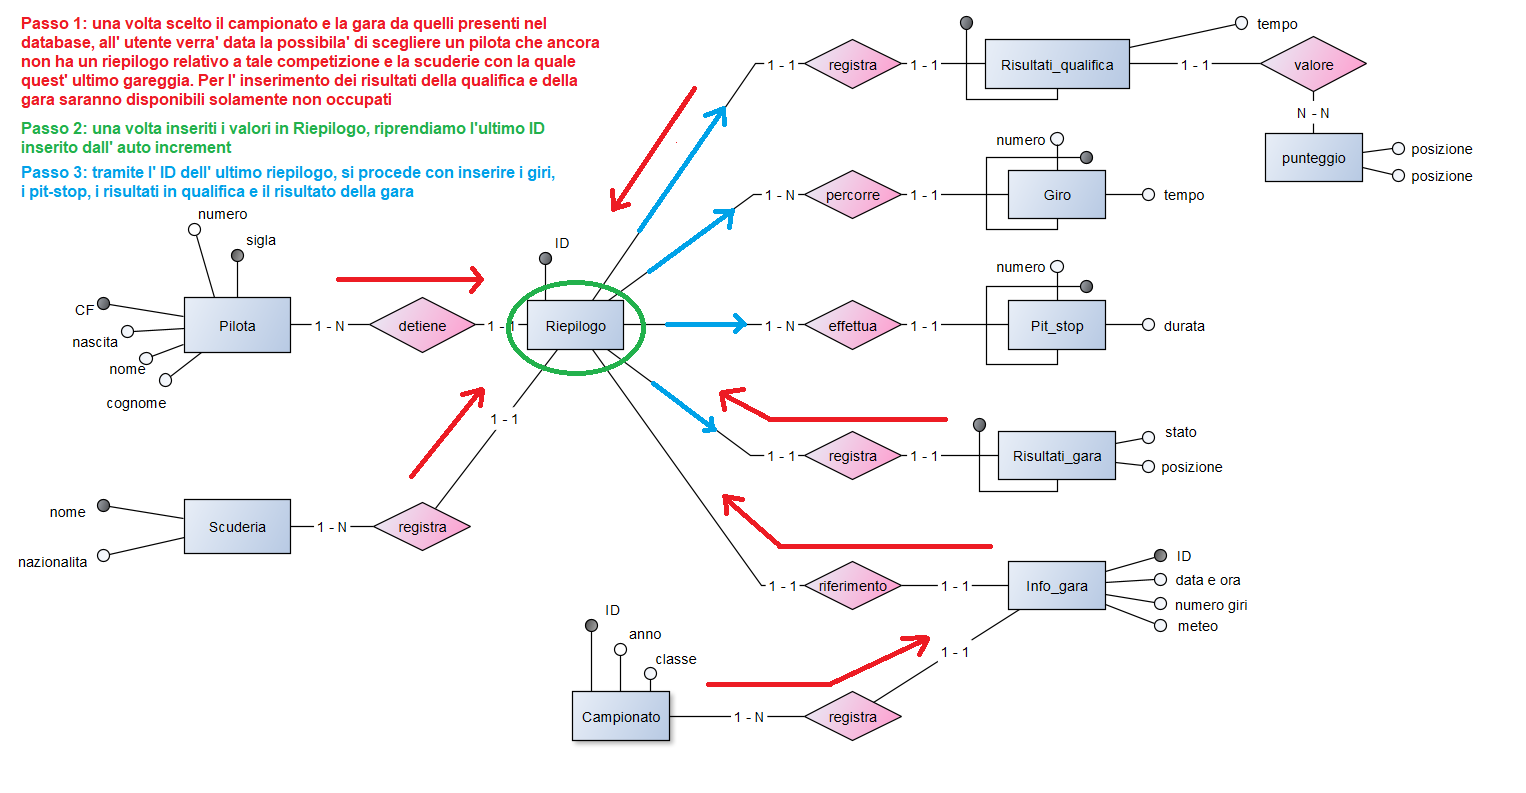
\includegraphics[width=\dimexpr\textwidth+10cm\relax, height=17cm, angle=90]{copies/navigazioneRiepilogo.png} 
					\hspace*{-4cm}%
				\end{center}
			\subsection{Classifica piloti nel campionato}
			{\fontsize{12.5}{20}\selectfont
			Una volta selezionato dall'utente un campionato, viene visualizzata la classifica dei piloti
			tenendo conto dei punteggi delle gare vinte e degli eventuali bonus derivati dai giri migliori.}
			\begin{table}[!htb]
				\centering
				\begin{center}
					\scalebox{1.2}{
						\begin{tabular}{|c|c|c|c|} % <-- Alignments: 1st column left, 2nd middle and 3rd right, with vertical lines in between
							\hline\rowcolor{Rosso}
							\toprule
							\textbf{Concetto} & \textbf{Costrutto} & \textbf{Accessi} & \textbf{Tipo}\\
							\midrule
							campionato  			& E & 1 	& L\\
							punteggi\_posizione		& E & 1		& L\\
							riepilogo 				& R & 2 	& L\\
							info\_gara				& E & 2 	& L\\
							risultati\_gara			& E & 1 	& L\\
							giro 					& E & 1 	& L\\
							\bottomrule
					\end{tabular}}
				\newline\\
				8L = 480 ogni anno\\
				\end{center}
			\end{table}\\
			\subsection{Classifica scuderie nel campionato}
			{\fontsize{12.5}{20}\selectfont
			Una volta selezionato un campionato, viene visualizzata la classifica delle scuderie.}
			\begin{table}[!htb]
				\centering
				\begin{center}
					\scalebox{1.2}{
						\begin{tabular}{|c|c|c|c|} % <-- Alignments: 1st column left, 2nd middle and 3rd right, with vertical lines in between
							\hline\rowcolor{Rosso}
							\toprule
							\textbf{Concetto} & \textbf{Costrutto} & \textbf{Accessi} & \textbf{Tipo}\\
							\midrule
							campionato  			& E & 1 	& L\\
							riepilogo 				& R & 2 	& L\\
							info\_gara				& E & 1 	& L\\
							risultati\_gara			& E & 2 	& L\\
							punteggi\_posizione		& E & 1		& L\\
							giro 					& E & 1 	& L\\
							\bottomrule
					\end{tabular}}
				\newline\\
				8L = 480 ogni anno\\
				\end{center}
			\end{table}\\
			\pagebreak
			\subsection{Numero vittorie di ogni pilota}
			{\fontsize{12.5}{20}\selectfont
			Viene visualizzato il numero di vittorie compiute da ogni pilota nella sua carriera.}
			\begin{table}[!htb]
				\centering
				\begin{center}
					\scalebox{1.2}{
						\begin{tabular}{|c|c|c|c|} % <-- Alignments: 1st column left, 2nd middle and 3rd right, with vertical lines in between
							\hline\rowcolor{Rosso}
							\toprule
							\textbf{Concetto} & \textbf{Costrutto} & \textbf{Accessi} & \textbf{Tipo}\\
							\midrule
							riepilogo 				& R & 1 	& L\\
							risultati\_gara			& E & 1 	& L\\
							\bottomrule
					\end{tabular}}
				\newline\\
				2L = 24 ogni anno\\
				\end{center}
			\end{table}\\
			\subsection{Classifica veicoli in una categoria}
			{\fontsize{12.5}{20}\selectfont
		Selezionata la categoria dei veicoli, viene visualizzata la classifica delle macchine più performanti in base al numero
		di giri migliori ottenuti nelle varie competizioni.}
		\begin{table}[!htb]
			\centering
			\begin{center}
				\scalebox{1.2}{
					\begin{tabular}{|c|c|c|c|} % <-- Alignments: 1st column left, 2nd middle and 3rd right, with vertical lines in between
						\hline\rowcolor{Rosso}
						\toprule
						\textbf{Concetto} & \textbf{Costrutto} & \textbf{Accessi} & \textbf{Tipo}\\
						\midrule
						campionato 				& E & 2 	& L\\
						giro 					& E & 1 	& L\\
						riepilogo 				& R & 1 	& L\\
						macchina 				& E & 1 	& L\\
						\bottomrule
				\end{tabular}}
			\newline\\
			5L = 50 ogni anno\\
			\end{center}
		\end{table}\\
		\begin{center}
				\hspace*{-2cm}%
				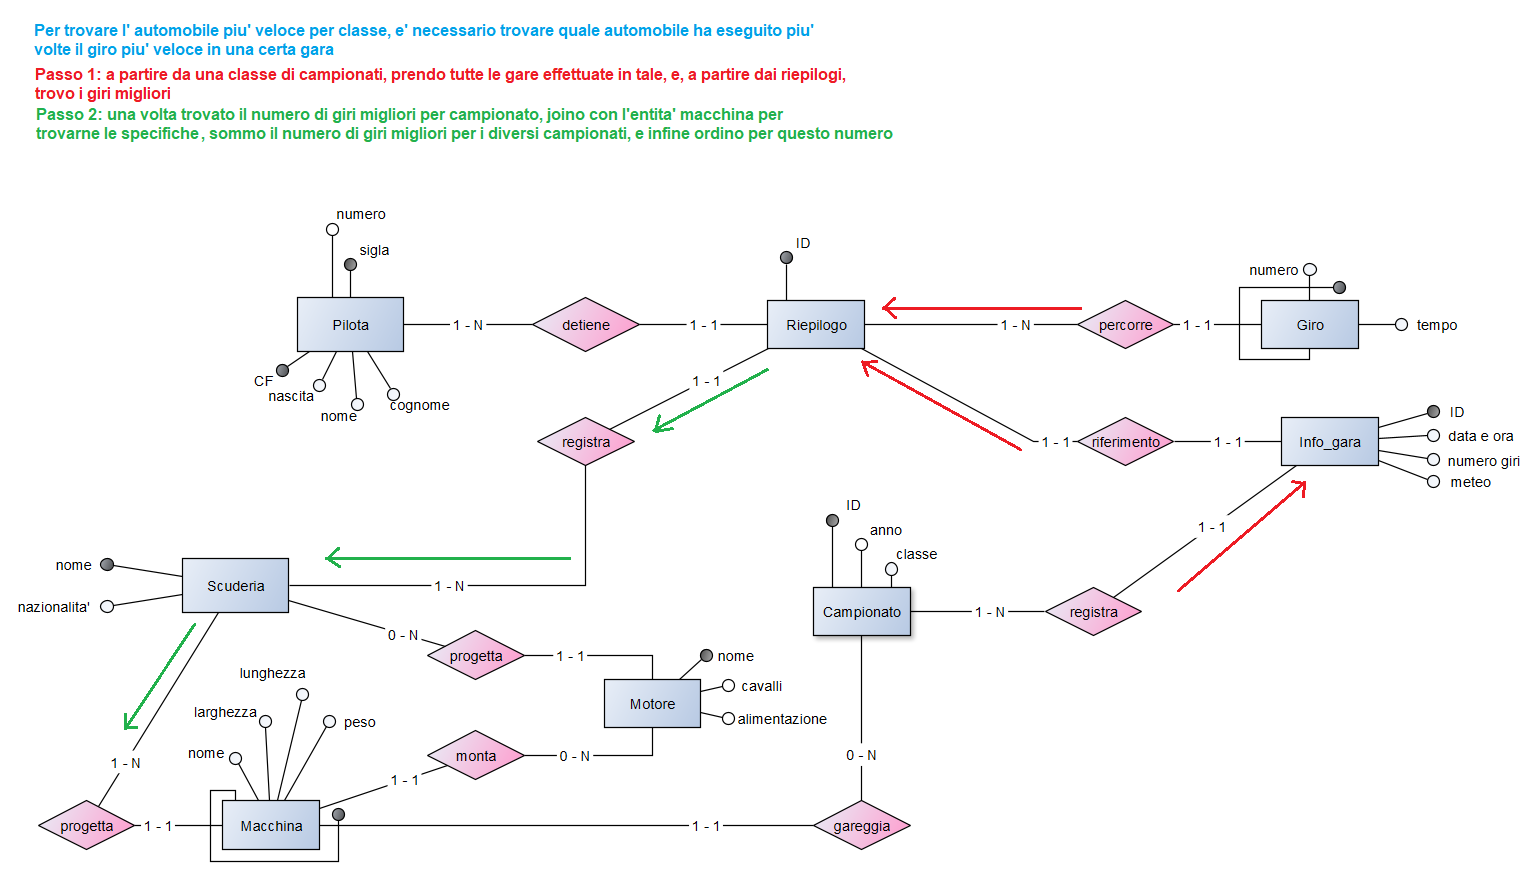
\includegraphics[width=\dimexpr\textwidth+10cm\relax, height=17cm, angle=90]{copies/navigazioneClassifica.png}%
				\hspace*{-4cm}%
			\end{center}
		\section{Analisi delle ridondanze}
			{\fontsize{12.5}{20}\selectfont{
			È stato introdotto l'attributo ridondante `posizione` all'entità risultati\_gara al fine di evitare i passi che coinvolgono il calcolo, quali, per esempio, la somma di tutti i tempi dei vari giri per calcolare in quanto tempo un pilota ha concluso una gara;	
			Questa ridondanza semplifica notevolmente tutte le query ove è necessario calcolare la posizione dei piloti.\\
			Esempio nella operazione: Classifica del campionato\\
			Lettura della posizione di un pilota in una gara.\\\\
			Con ridondanza:}
			\begin{table}[h!]
				\centering
				\begin{center}
					\scalebox{1.2}{
						\begin{tabular}{|c|c|c|c|} % <-- Alignments: 1st column left, 2nd middle and 3rd right, with vertical lines in between
							\hline\rowcolor{Rosso}
							\toprule
							\textbf{Concetto} & \textbf{Costrutto} & \textbf{Accessi} & \textbf{Tipo}\\
							\midrule
							campionato 			& E & 1 & L\\
							punteggio\_posizione & E & 1 & L\\
							riepilogo 			& R & 2 & L\\
							info\_gara 			& E & 1 & L\\
							risultati\_gara 	& E & 1 & L\\
							giro 				& E & 1 & L\\
							\bottomrule
					\end{tabular}}
				\newline\\
				7L = 420 ogni anno\\
				\end{center}
			\end{table}\\
			{\fontsize{12.5}{20}\selectfont
			Senza ridondanza:}
			\begin{table}[h!]
				\centering
				\begin{center}
					\scalebox{1.2}{
						\begin{tabular}{|c|c|c|c|} % <-- Alignments: 1st column left, 2nd middle and 3rd right, with vertical lines in between
							\hline\rowcolor{Rosso}
							\toprule
							\textbf{Concetto} & \textbf{Costrutto} & \textbf{Accessi} & \textbf{Tipo}\\
							\midrule
							campionato 				& E & 1 	& L\\
							punteggio\_posizione 	& E & 1 & L\\
							riepilogo 				& R & 2 	& L\\
							info\_gara 				& E & 1 	& L\\
							giro 					& E & 21 	& L\\
							\bottomrule
					\end{tabular}}
				\newline\\
				26L = 1560 ogni anno\\
				\end{center}
			\end{table}
		\section{Raffinamento dello schema}
			{\fontsize{12.5}{20}\selectfont
			\textbf{Eliminazione delle gerarchie:}\\
				Per l'eliminazione della gerarchia 'Persona' si è scelto di adottare l'approccio del collasso verso il basso,
				inserendo in Ingegnere e in Pilota gli attributi prima appartenenti al padre.
				La scelta di questo approccio deriva dalla presenza dell'associazione tra Pilota e Riepilogo, la più importante dello schema, e in quanto le interazioni con i piloti sono molto più frequenti rispetto a quelle con gli ingegneri.
			\\\\
			\textbf{Scelta delle chiavi primarie:}\\
				Le chiavi primarie selezionate sono rimaste quasi completamente fedeli a quelle definite nello schema ER,
				a differenza dell'identificatore di Riepilogo, sostituito da un numero intero per facilitarne il successivo utilizzo
				in chiavi esterne; per lo stesso motivo, anche per le entità info\_gara e campionato è stato scelto come identificatore
				una cifra numerica.
				All'entità pilota è stata inoltre rimossa la chiave primaria CF, in quanto non più necessaria e per rendere
				più significativi i valori della tabella riepilogo, memorizzando il pilota con la sua sigla al posto che il codice fiscale.}
		\pagebreak
		\section{Traduzione delle entità e associazioni in relazioni}
			{\fontsize{12.5}{20}\selectfont
			Sono state eliminate le seguenti relazioni:
			\lstset{language={},
					basicstyle=\small\ttfamily,
					columns=fullflexible,
					keywords=[2]{fail},
					keywords=[3]{pass},
					keywordstyle={\color{blue!80!black}},
					keywordstyle=[2]{\color{red!80!black}},
					keywordstyle=[3]{\color{green!50!black}},}
			\begin{lstlisting}[language={}]
provenienza: 										importando nazione.sigla in Ingegnere 
			  	e Pilota, una volta rimossa la gerarchia
appartenenza: 									importando nazione.sigla in Scuderia
contratto: 												reificando l'associazione importando CF 
			  	da ingegnere e nome da scuderia
stipula, riguarda: 				importando pilota.sigla e scuderia.nome 
			  	in contratto_pilota
costruisce, gareggia: 	importando campionato.ID e scuderia.nome 
			  	in macchina
progetta: 													importando scuderia.nome in motore
monta: 																importando motore.nome in macchina
locazione: 												importando nazione.sigla in circuito
svolgimento: 										importando circuito.nome in info_gara
compone: 														importando campionato.ID in info_gara
detiene: 														importando pilota.sigla in riepilogo
lega:																		importando scuderia.nome in riepilogo
percorre:														importando riepilogo.ID in giro
effettua:														importando riepilogo.ID in pit_stop
segna:																	importando riepilogo.ID in risultati_gara
registra:														importando riepilogo.ID in risultati_qualifica
valore:																importando punteggio.valore in risultati_gara
			\end{lstlisting} \par\noindent\rule{\textwidth}{0.4pt}
			\textbf{nazione}(\underline{sigla}, nome)\\
			\textbf{campionato}(\underline{ID}, anno, classe)\\
			\textbf{circuito}(\underline{nome}, lunghezza, nazione:nazione, città)\\
			\textbf{scuderia}(\underline{nome}, nazionalità:nazione)\\
			\textbf{motore}(\underline{nome}, produttore:scuderia, cavalli, alimentazione)\\
			\textbf{macchina}(\underline{ID\_scuderia}:scuderia, \underline{ID\_campionato}:campionato, 
			\tab\tab motore:motore, peso, lunghezza, larghezza)\\
			\textbf{pilota}(\underline{sigla}, numero, nazionalità:nazione, nascita, nome, cognome)\\
			\textbf{contratto\_pilota}(\underline{ID\_pilota}:pilota, \underline{ID\_scuderia}:scuderia, data\_inizio, \tab\tab durata\_anni)\\
			\textbf{punti\_posizione}(\underline{posizione}, punteggio)\\
			\textbf{ingegnere}(\underline{CF}, specialità, nazionalità:nazione, nascita, nome, cognome)\\
			\textbf{contratto}(\underline{CF}:ingegnere, \underline{ID\_scuderia}:scuderia)\\
			\textbf{info\_gara}(\underline{ID}, data\_gara, n\_giri, meteo, circuito:circuito, campionato:campionato)\\
			\textbf{riepilogo}(\underline{ID}, gara:info\_gara, pilota:pilota, scuderia:scuderia)\\
			\textbf{giro}(\underline{ID\_riepilogo}:riepilogo, \underline{numero}, tempo)\\
			\textbf{risultati\_gara}(\underline{ID\_riepilogo}:riepilogo, posizione:punti\_posizione, stato)\\
			\textbf{risultati\_qualifica}(\underline{ID\_riepilogo}:riepilogo, posizione, tempo)\\
			\textbf{pit\_stop}(\underline{numero}, \underline{ID\_riepilogo}:riepilogo, durata)\\}
		\section{Schema relazionale finale}
			\pagebreak
			\begin{center}
							\hspace*{-2cm}%
							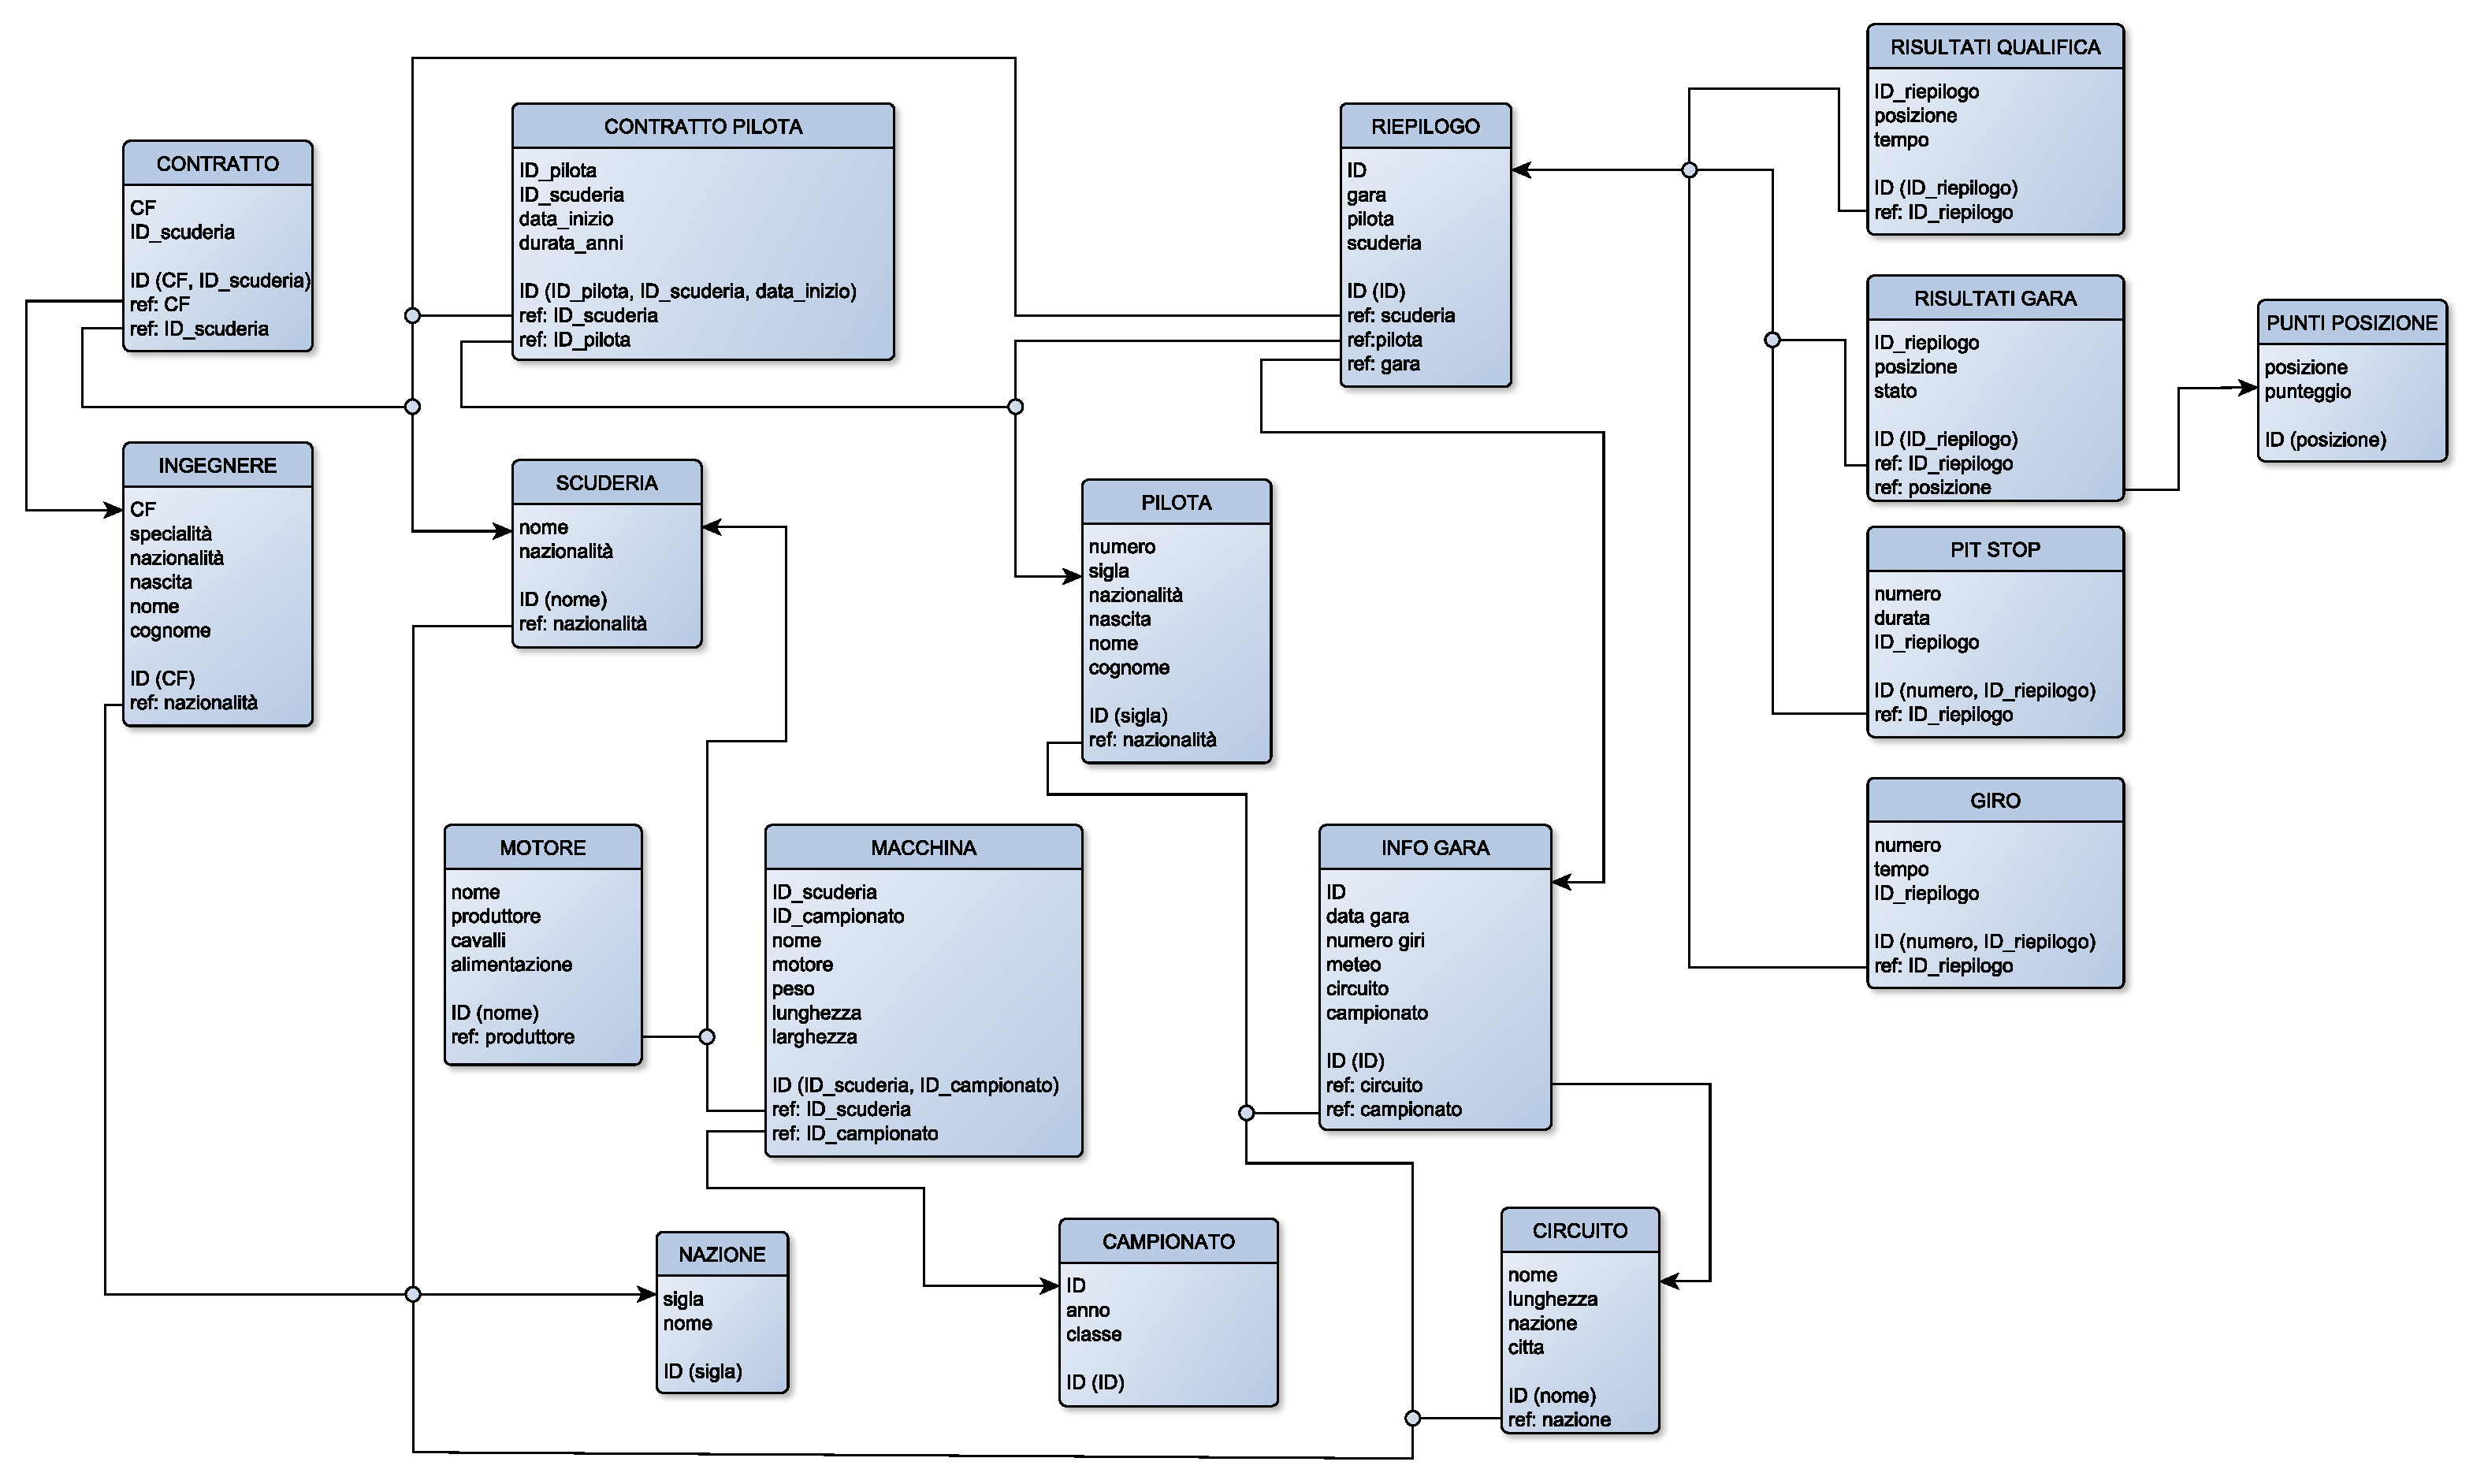
\includegraphics[width=\dimexpr\textwidth+7cm\relax, height=17cm, angle=90]{copies/schemaFinale.pdf}%
							\hspace*{-8cm}%
						\end{center}
					\pagebreak
		\section{Traduzione delle operazioni in query SQL}
			\lstset{
				language=SQL,
				basicstyle=\small\ttfamily,
				columns=fullflexible,
				keywords=[2]{fail},
				keywords=[3]{pass},
				keywordstyle={\color{blue!80!black}},
				keywordstyle=[2]{\color{red!80!black}},
				keywordstyle=[3]{\color{green!50!black}},
			}
			\begin{adjustwidth}{-85pt}{1pt}
			\begin{lstlisting}[language=SQL]
01 - aggiunta di un motore
select * from scuderia;
insert into motore (nome, produttore, cavalli, alimentazione) values ('?', '?', ?, '?');


02 - aggiunta di una scuderia
select * from nazione;
insert into scuderia (nome, nazionalita) values ('?', '?');


03 - aggiunta di un pilota
select * from nazione;
select * from scuderia;
insert into pilota (numero, sigla, nazionalita, nascita, nome, cognome) 
		value (?, '?', '?', '?', '?', '?');
insert into contratto_pilota(ID_pilota, ID_scuderia, data_inizio) values('?', '?', '?', ?);


04 - aggiunta di una macchina ad una scuderia
select * from campionato;
select * from motore;
select * from scuderia;
insert into macchina (ID_scuderia, ID_campionato, nome, motore) values ('?', ?, '?', '?');


05 - aggiunta di un circuito
select * from nazione;
insert into circuito (lunghezza, nome, nazione, citta) values (?, '?', '?', '?');


06 - aggiunta di un campionato
insert into campionato (anno, classe) values (?, '?');


07 - aggiunta di una gara ad un campionato
select * from campionato;
select * from circuito;
insert into info_gara (data_gara, n_giri, meteo, circuito, campionato) values ('?', ?, '?', '?', ?);




08 - aggiungere il riepilogo di un pilota
select * from campionato;
select * from info_gara where campionato = ?;
	-- guardo quali piloti non hanno una entry nella gara scelta
select * from pilota where pilota.sigla not in (select Riepilogo.pilota as numero 
						     from riepilogo 
						     where gara = ?);
	-- prendo le posizione non occupate
select posizione from risultati_gara where ID_riepilogo in (select ID as ID_riepilogo 
								   from riepilogo where gara = ?);
select posizione from risultati_qualifica where ID_riepilogo in (select ID as ID_riepilogo 
									from riepilogo where gara = ?);										
select * from scuderia;
select ID_scuderia from Contratto_pilota where ID_pilota = '?';
	-- inserisco i dati
insert into riepilogo(gara, pilota, scuderia) values(?, '?', '?');
select max(ID) from Riepilogo; -- si potrebbe anche usare LAST_INSERT_ID() nei campi ID_riepilogo
insert into Risultati_qualifica (ID_riepilogo, posizione, tempo) values (?, ?, '?');
insert into Risultati_gara (ID_riepilogo, posizione, stato) values (?, ?, '?');
-- da eseguire per ogni pit stop
insert into Pit_stop(numero, durata, ID_riepilogo) values(?, '?', ?);	
-- da eseguire per ogni giro
insert into giro(numero, tempo, ID_riepilogo) values(?, '?', ?);			
	
	
09 - visualizzare la classifica dei piloti in un campionato
select res1.pilota, punteggio + IFNULL(girimigliori, 0) as punteggio from
	-- punti dati dalle posizioni in gara
	(select pilota, sum(punteggio) as punteggio from (
		select gara, pilota, posizione as pos
		from (riepilogo join info_gara on riepilogo.gara = info_gara.ID join risultati_gara 
						on risultati_gara.ID_riepilogo = riepilogo.ID)
		where campionato = ?) as res
		join punti_posizione on punti_posizione.posizione = res.pos
	group by pilota
	order by punteggio desc ) as res1

	left join 
	
	
	
	
	-- punti dati dai giri migliori
	(select pilota, count(*) as girimigliori from 
		(select * 
		from (
			select ID_riepilogo, gara, pilota ,scuderia ,min(tempo) as best
			from giro join riepilogo on riepilogo.ID = giro.ID_riepilogo  join info_gara 
						on info_gara.ID = riepilogo.gara
			where info_gara.campionato = ?
			group by gara, pilota
			order by gara, best ) as res
		group by gara ) as res2
	group by pilota) as res2

	on res1.pilota = res2.pilota;

	
10 - visualizzare la classifica delle autombili
select res1.scuderia, punteggio + IFNULL(girimigliori, 0) as punteggio from 
	-- punti dati dalle posizioni in gara
	( select scuderia, sum(punteggio) as punteggio
	from (riepilogo join info_gara on riepilogo.gara = info_gara.ID join risultati_gara 
				on risultati_gara.ID_riepilogo = riepilogo.ID join punti_posizione 
				on risultati_gara.posizione = punti_posizione.posizione)
	where campionato = ? 
	group by scuderia) as res1

	left join 
	-- punti dati dai giri migliori
	(select scuderia, count(*) as girimigliori from ( -- migliore giro per scuderia
		select *
		from (
			select ID_riepilogo, gara, pilota ,scuderia ,min(tempo) as best
			from giro join riepilogo on riepilogo.ID = giro.ID_riepilogo join info_gara 
								on info_gara.ID = riepilogo.gara
			where info_gara.campionato = ?
			group by gara, pilota
			order by gara, best ) as res
		group by gara ) as res
	group by scuderia) as res2

	on res1.scuderia = res2.scuderia
	order by punteggio desc;

	
11 - visualizzare il numero di vittorie di ogni pilota
select riepilogo.pilota, nome, cognome, numero, count(*) as vittorie
from riepilogo join Risultati_gara on Riepilogo.ID = risultati_gara.ID_riepilogo join pilota 
								on pilota.sigla = riepilogo.pilota
where risultati_gara.stato = 'END' and risultati_gara.posizione = 1
group by riepilogo.pilota
order by vittorie desc;


12 - ottenere la classifica dei veicoli piu veloci per classe a partire dal numero di giri migliori
select scuderia, sum(bestlaps) as girimigliori, nome, motore, peso, lunghezza, larghezza from (
	select scuderia, count(*) as bestlaps, campionato from (
		select * from(
			select ID_riepilogo, gara, pilota ,scuderia ,min(tempo) as best, campionato
			from giro join riepilogo on riepilogo.ID = giro.ID_riepilogo join info_gara 
							on info_gara.ID = riepilogo.gara join campionato 
							on campionato.ID = info_gara.campionato
			where campionato.classe = '?'
			group by gara, pilota
			order by gara, best ) as res
		group by gara ) as res
	group by scuderia ) as res
	join macchina on macchina.ID_scuderia = res.scuderia 
			and macchina.ID_campionato = res.campionato
	group by nome
	order by bestlaps desc;
	
	
13 - ottenere il giro piu veloce di ogni circuito
select circuito.nome, min(giro.tempo) as 'miglior tempo'
	from circuito join info_gara on (circuito.nome = info_gara.circuito) join riepilogo 
				on (info_gara.id = riepilogo.gara) join giro 
				on (riepilogo.id = giro.ID_riepilogo)
	group by circuito.nome;

			\end{lstlisting}
			\end{adjustwidth}
\chapter{Progettazione dell'applicazione}
		{\fontsize{12.5}{20}\selectfont
		\section{Descrizione dell'architettura dell'applicazione realizzata}
			L'applicazione per interfacciarsi al database è realizzata in C\#, utilizzando il framework
			WPF per la creazione di pagine con la quale l'utente è in grado in interagire.
			Il DBMS scelto e' MySql.\\
			All'avvio del programma l'utente potrà scegliere quale operazione effettuare cliccando uno dei 12 bottoni 
			presenti nella schermata; ogni operazione sarà svolta su una finestra assestante e la correttezza dei dati obbligatori
			sarà garantita da controlli eseguiti da codice a runtime (ad esempio se una casella di testo non è stata riempita) e 
			da messaggi visualizzati all'utente sotto forma di pop-up in caso di errore nell'operazione.
			\par\noindent\rule{\textwidth}{0.4pt}
			\begin{center}
								\hspace*{-1cm}%
								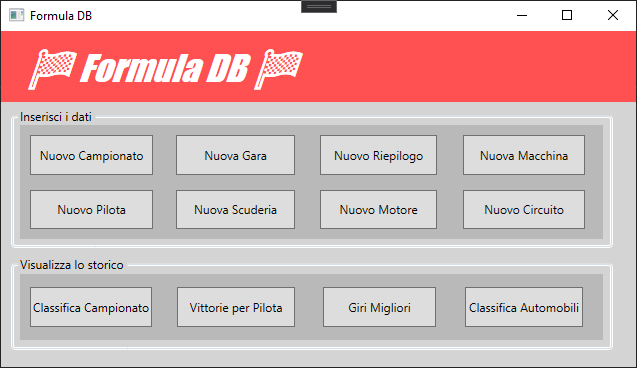
\includegraphics{copies/gui.png} 
								\hspace*{-4cm}%
							\end{center}
			\pagebreak
			\subsection{Operazioni di inserimento}
				Tramite le operazioni di inserimento l'utente è in grado di inserire tutti i dati necessari per riguardare ogni aspetto di un campionato.
				\subsubsection{Aggiunta di un riepilogo}
					L'inserimento del riepilogo di una gara per un certo pilota e' un processo che richiede vari passaggi:
					inizialmente l'utente dovrà scegliere un campionato tra i disponibili ed in seguito la gara della quale si desidera registrare
					l'ennupla.
					Una volta selezionata la gara dall'apposita tabella, verrà data la possibilità di selezionare un pilota tra quelli 
					ai quali non risulta ancora un riepilogo nella gara selezionata in precedenza, e una volta selezionato il gareggiante,
					sarà inoltre possibile scegliere la scuderia per la quale gareggia; quella di contratto viene selezionata di default;
					Per completare l'operazione sarà inoltre necessario impostare la posizione guadagnata in qualifica e in gara, selezionabile
					dalle opportune combobox tra quelle non occupate, e specificare i tempi dei vari giri e pit-stop.
					\begin{center}
							\hspace*{-1cm}%
							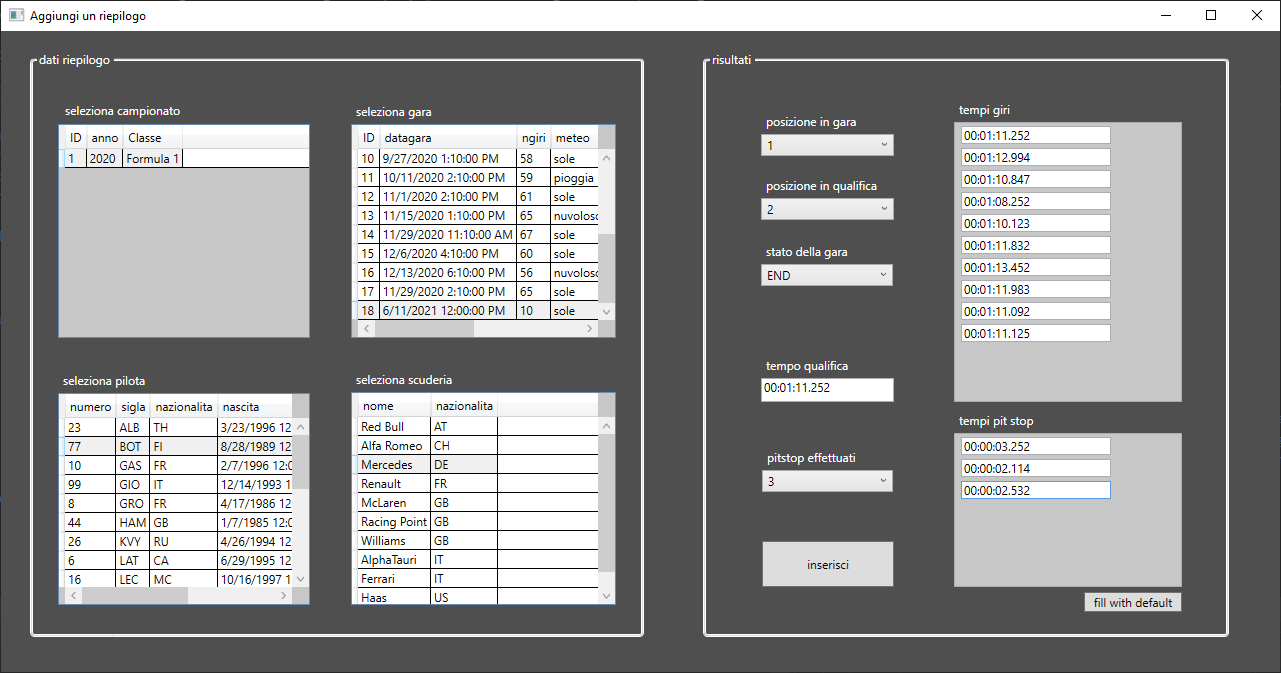
\includegraphics[scale=0.57, angle=90]{copies/riepilogo.png} 
							\hspace*{-4cm}%
					\end{center}
			\subsection{Operazioni di visualizzazione}
				Per tutte le operazioni sotto la voce "visualizza lo storico", l'utente non dovrà inserire dati ma scegliere solamente
				cosa visualizzare, nell'esempio riportato, una volta premuto il bottone "Giri Migliori" nella schermata principale, sei aprirà una nuova
				finestra contenenti i giri più veloci effettuati in tutti i circuiti registrati
				\begin{figure}[htbp]
					\centering
					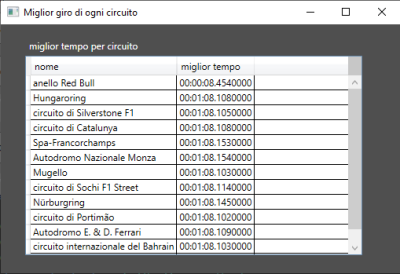
\includegraphics[scale=1]{copies/risultati.png}
				\end{figure}
				}
\end{document}